\documentclass{article}
\usepackage{pgfplots}
\pgfplotsset{compat=1.17}

\begin{document}

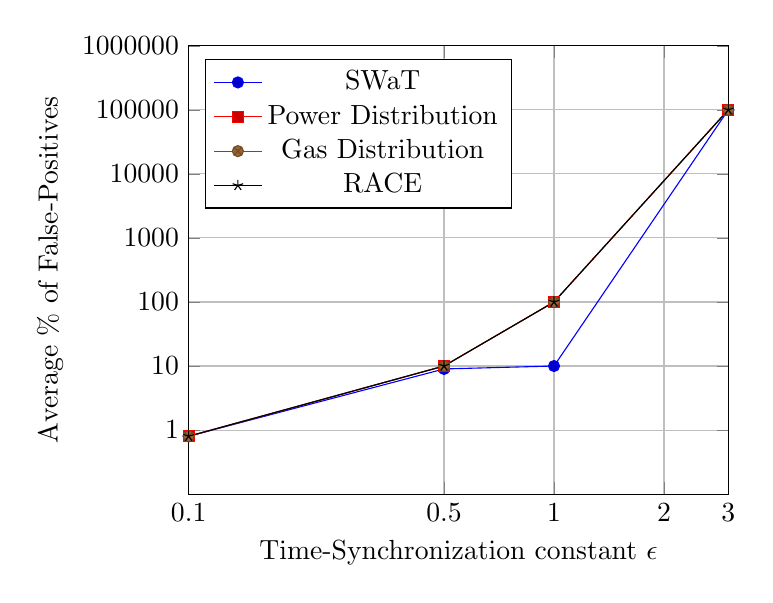
\begin{tikzpicture}
    \begin{loglogaxis}[
        xlabel={Time-Synchronization constant $\epsilon$},
        ylabel={Average \% of False-Positives},
        legend pos=north west,
        legend entries={SWaT, Power Distribution, Gas Distribution, RACE},
        log basis x={10},
        log basis y={10},
        grid=major,
        ymin=0.1,
        ymax=1000000,
        xmin=0.1,
        xmax=3,
        ytick={1, 10, 100, 1000, 10000, 100000, 1000000},
        yticklabels={\(1\), \(10\), \(100\), \(1000\), \(10000\), \(100000\), \(1000000\)},
        xtick={0.1, 0.5, 1, 2, 3},
        xticklabels={\(0.1\), \(0.5\), \(1\), \(2\), \(3\)},
    ]
        
        % SWaT data points
        \addplot coordinates {
            (0.1, 0.8)
            (0.5, 9)
            (1, 10)
            (3, 100000)
        };
        
        % Power Distribution data points
        \addplot coordinates {
            (0.1, 0.8)
            (0.5, 10)
            (1, 100)
            (3, 100000)
        };
        
        % Gas Distribution data points
        \addplot coordinates {
            (0.1, 0.8)
            (0.5, 10)
            (1, 100)
            (3, 100000)
        };
        
        % RACE data points
        \addplot coordinates {
            (0.1, 0.8)
            (0.5, 10)
            (1, 100)
            (3, 100000)
        };
        
    \end{loglogaxis}
\end{tikzpicture}

\end{document}